\documentclass[twoside,10pt]{book}
\usepackage{graphicx}
\usepackage{hyperref}
\usepackage{xcolor}
\usepackage[utf8]{inputenc}

%----------------------------------------------------------------------------------------
%	MACROS
%----------------------------------------------------------------------------------------

\newcommand{\pror}[0]{ProR}

%----------------------------------------------------------------------------------------
%	ENVIRONMENTS
%----------------------------------------------------------------------------------------

\definecolor{color-info}{RGB}{0,0,128} 
\newenvironment{info}{\begin{description}\item[\textcolor{color-info}{Information.}]}{\end{description}}

\definecolor{color-warning}{RGB}{128,0,0} 
\newenvironment{warning}{\begin{description}\item[\textcolor{color-warning}{Warning.}]}{\end{description}}

\newsavebox{\mybox}
\newenvironment{example}
{\begin{lrbox}{\mybox}\begin{minipage}{0.9\textwidth}}
{\end{minipage}\end{lrbox}\fbox{\usebox{\mybox}}}

%----------------------------------------------------------------------------------------
%	DOCUMENT INFO
%----------------------------------------------------------------------------------------

\title{Eclipse ProR}
\author{by the RMF Community}

%----------------------------------------------------------------------------------------
%	START DOCUMENT
%----------------------------------------------------------------------------------------

\begin{document}        

\maketitle

\chapter{Introduction}
\pror{} is the user interface of the Eclipse Requirements Modeling Framework.  This handbook strives to be a complete reference for \pror{}.  Included is a tutorial making it as easy as possible for new users to get started with requirements engineering.

\section{Conventions}

Throughout this book you'll see the following conventions:

% Formatted like remark
\begin{info}
This is where you'll find useful information or tips.
\end{info}

\begin{warning}
This will mark things to be aware of.
\end{warning}

\begin{example}
Examples will be marked as such.
\end{example}


When referring to \menu{menus} or \menu{user interface elements}, they are marked as shown here.
%\begin{definition}[Definition name]
%This is a definition
%\end{definition}


\section{Contributing}

Documentation is one of those things that gets easily neglected in open source projects.  It is also one of the easiest for outsiders to contribute to.  The documentation is managed as \LaTeX, which may scare some people.  But no worries, those who don't want to learn \LaTeX don't have to.

There are broadly two ways for contributing to the documentation:

\begin{description}
  \item[File a bug.]  Visit the \href{https://bugs.eclipse.org/bugs/enter_bug.cgi?assigned_to=&blocked=&bug_severity=normal&bug_status=NEW&comment=&contenttypeentry=&contenttypemethod=autodetect&data=&dependson=&description=&flag_type-1=X&flag_type-11=X&flag_type-12=X&flag_type-2=X&flag_type-4=X&flag_type-6=X&flag_type-7=X&flag_type-8=X&form_name=enter_bug&keywords=&&op_sys=All&product=MDT.RMF&qa_contact=&rep_platform=All&short_desc=&version=unspecified}{RMF Bug Tracker}.  You can just point out a problem or request for improvement.  You can also provide some text to be added to the documentation (unformatted).  If you do, however, then you need to sign a Committer License Agreement (CLA)
  \item[Submit improved \LaTeX via Gerrit.]  If you are technically inclined (meaning that you know what \LaTeX and git are, and how to use them), then you can contribute via the Gerrit code review system, as described \href{https://wiki.eclipse.org/Gerrit}{at eclipse.org}.
\end{description}

\subsection{Gerrit for Contributions}

TODO - when done, update the parent section as well.

\section{Licensed as EPL}

This work is licensed under the Eclipse Public License.

\section{Acknowledgements}

Many parties were involved in the creation of RMF.  We would like to thank the core team that made it possible.

\begin{figure}[H]
  \centering
  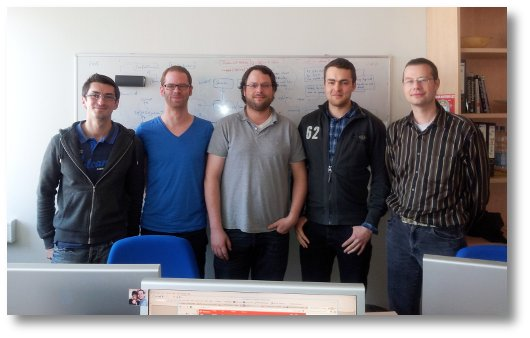
\includegraphics[width=\textwidth]{../rmf-images/2012_03_sprint_team.jpg}
  \caption{The RMF team during a Sprint in April 2012 in Düsseldorf, Germany (left to right) Lukas Ladenberger, Mark Brörkens, Ingo Weigelt, Said Salem, Michael Jastram}
  \label{fig:intro_core_team}
\end{figure}


The roots of this project were created by Andreas Graf, Michael Jastram and Nirmal Sasidharan, who joined together individual projects to create RMF.  Their efforts were financed by the research projects itea Verde and FP7 Deploy.  RMF was assembled at the Eclipse Foundation, where it has been active ever since.  Figure~\ref{fig:intro_core_team} shows four of the five RMF Committers at a joint coding session (missing is Andreas Graf).


\chapter{Tutorial}
\section{Basic ReqIF Concepts}

A ReqIF model is a structured collection of natural language
requirements. However, it comes with its own terminology. For instance,
a ``Requirement'' is called ``SpecObject'' in ReqIF:

A ReqIF model has some similarities to a Excel Spreadsheet, although
there are some notable differences. It's simply meant as a starting
point to get a feel for ReqIF.

The following table compares a Spreadsheet model with a ReqIF model,
introduces the terminology and explains it:

\begin{description}
  \item[Specification.] (Excel-equivalent: Sheet)  A ReqIF model
consists of an arbitrary number of Specifications. The Specification is
the ``Container'' for the Requirements. Think of an Excel Document, that
allows you to create an arbitrary number of Sheets. There are two
differences to Excel: (1) The requirements in the Specification are
references (which means that the same requirement can appear in multiple
places); (2) The content of Specification is hierarchical.

  \item[SpecObject.] (Excel-equivalent: Row) A SpecObject represents the actual
Requirement. A requirement typically has a number Attributes. Again
compared with Excel, each row in a Sheet represents a requirement. In
contrast to Excel, the ReqIF model may contain SpecObjects that do not
appear in any Specification (whether this is useful is a different
question).

  \item[Attribute.] (Excel-equivalent: Cell) Besides the actual text of the
requirement, typical Attributes include ID, Status, etc. Note that there
are no ``standard'' Attributes. The ReqIF model contains the definitions
of the Attributes. Here the Excel analogy starts to break down. In
Excel, each row has the same columns. Different SpecObjects may have
different sets of Attributes.

  \item[SpecType.] (Excel-equivalent: Column configuration) Each SpecObject
has a SpecObjectType. The SpecObjectType contains a list of Attributes
for the SpecObject. For instance, the SpecObjectType ``Headline'' may
have only one Attribute ``HeadlineText''. Another SpecObjectType
``Requirement'' may have three Attributes, ``ID'', ``Description'' and
``Status''. A Specification may then contain a mixture of SpecObjects
with different types.

\end{description}

There are many more concepts, but this is enough to get us started.

Let's look at a concrete example to understand this. Here is a snippet
of a Specification:

The table shows the first four SpecObjects, as visualized in a
Specification. The tree-like structure is recognizable: INF-1 is a node
with three children, REQ-1, REQ-2 and REQ-3 (this can be seen by the
indentation). Let's look at INF-1 and REQ-1. If they would be selected
in the GUI, the Property pane would show their Attributes, as it is
shown to the right.

INF-1 has two attributes, ``Description'' and ``ID''. The SpecObjectType
is ``Information Type'' (shown as the root in the properties view).

REQ-1 has three attributes, ``Description'', ``ID'' and ``Status''. The
SpecObjectType is called ``Requirements Type''. Let's have a closer look
at that one.

The ``Requirements Type'' SpecObjectType is shown in the picture, with
arrows indicating how the Attributes relate to the SpecObjectType (a
simple one-to-one relationship). A SpecObjectType has one entry for each
Attribute, consisting of a name and a Datatype. For instance, the first
entry has the name ``ID'' and the datatype ``T\_ID\_REQ''. Note that
multiple Attributes may have the same Datatype: ``Description'' and
``Status'' both have the Datatype ``T\_String32k''.

Last, The Datatypes must be defined as well. In this example, there are
two Datatypes, ``T\_String32'' and ``T\_ID\_REQ''. These are finally
based on a number of standard types that ReqIF supports.

NOTE: As of this writing, we only implemented the simple and the
enumeration ReqIF types. This leaves out the complex ones (rich text,
attachments, embedded files, etc.) for now.

\section{Tutorial 1: Creating a basic ReqIF Model}

In this Section, we will build a ReqIF model from scratch, step by step.

\subsection{Install \pror{}}

You can download \pror{} from the
\href{http://www.eclipse.org/rmf/download.php}{Download page}.
Alternatively, you can install \pror{} in any Eclipse-Installation via its
update site (also listed on the
\href{http://www.eclipse.org/rmf/download.php}{Download page}). Using
the update site allows you to use the Eclipse Update mechanism,
something that is currently not yet enabled for the standalone version.

\subsection{Create the Model}

\begin{itemize}

\item
  Make sure that you have at least one Project in the Workspace;
\item
  Select File \textgreater{} New \textgreater{} Reqif10 Model;
\item
  Select a Project and name the file (ending in .reqif), then click
  ``Finish'';
\item
  In the Window named ``file.reqif'', double-click on ``Requirements
  Document'' button in the ``Specifications'' panel.
\end{itemize}

After this, your window should look more or less as follows:

\begin{figure}[h!]
  \centering
  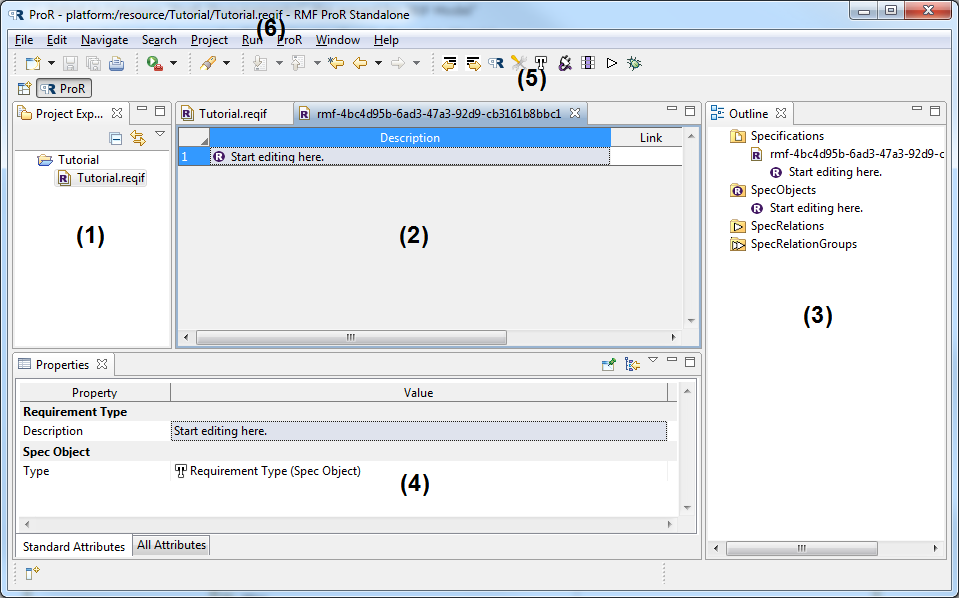
\includegraphics[width=\linewidth]{../rmf-images/pror-screenshot.png}
  \caption{The \pror{} user interface}
  \label{fig:user_interface_overview}
\end{figure}

You will see your ReqIF file in the (1) Project Explorer or the regular
Navigator.

The Editor (2) shows your Specifications.

In the Editor, you see the SpecObjects that exist in this Specification.
There is currently only one, with the description ``Start Editing''.

The Outline (3) has three folders:

\begin{itemize}

\item
  ``Specifications'' shows the Specifications in the ReqIF. You can
  expand the tree to expose the hierarchy of SpecObjects in the
  Specification.
\item
  ``SpecObjects'' shows all SpecObjects in the ReqIF as a flat list.
  Keep in mind that SpecObjects in Specifications are references. In
  contrast, this folder shows all SpecObjects in the ReqIF model, no
  matter whether they appear in any Specification.
\item
  ``SpecRelations'' shows all SpecRelations in the ReqIF as a flat list.
  For now, we will ignore SpecRelations.
\end{itemize}

The properties of a selected Element are shown in the Properties view
(4). As the only Requirement in the model is selected, we see its
SpecObjectType (``Requirements Type'') and its only Attribute
(``Description'') with the value ``Start editing here.''. There are two
tabs ``Standard Attributes'' and ``All Attributes'' at the bottom of the
Properties view. The ``Standard Attributes'' tab shows you all standard
attributes of the selected element. The ``All Attributes'' shows all
existing ReqIF attributes of the selected element.

When a ReqIF Editor is active, there are also additional tool bar items
(5) and an additional menu (6).

\subsection{Customizing the SpecType}

To get familiar with the system, next we will:

\begin{itemize}

\item
  Add two more attributes to the SpecObjectType called ``ID'' and
  ``Owner''
\item
  We will show those Attributes in the Specification
\end{itemize}

To add new attributes, we open the Datatype Configuration dialog with
\pror{} \textgreater{} Datatype Configuration.

The resulting Dialog has a folder for SpecTypes and Datatypes.
Currently, there is only one Datatype (T\_String32k) and two SpecTypes,
one called ``Requirements Type'' with one Attribute ``Description'' and
one called ``Specification Type'' with one Attribute ``Description''.

We add more Attributes to ``Requirements Type'' by right-clicking
``Requirements Type'' and selecting ``New Child \textgreater{} Attribute
Definition String''. This will create a new element. Upon selecting, we
can rename it in the lower pane. We do this twice for ``ID'' and
``Owner''. We assign both Attributes the same Datatype,
``T\_String32k''. In the end, the dialog should look as follows:

\begin{figure}[h!]
\centering
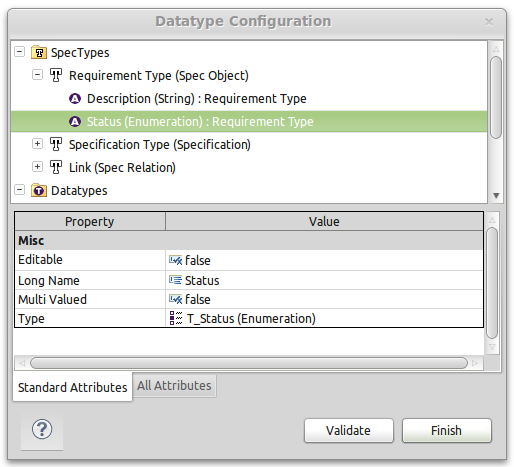
\includegraphics[width=0.8\linewidth]{../rmf-images/pror_datatype_configuration.png}
\caption{Datatype Configuration Dialog}
\label{fig:datatype_configuration}
\end{figure}

Upon closing the dialog, little will have changed - the Specification
still shows just two columns, Description and Link. However, if you
select the requirement, you will see the new Properties (ID and Owner)
in the Property view.

\subsection{Showing the new Attributes in the Specification}

To show the new Attributes in the Specification, we have to configure
the Specification columns. We do this by selecting \pror{} \textgreater{}
Column Configuration.

The resulting Dialog shows one entry for the one and only Column of the
Specification. By clicking on the ``Add Column'' icon at the top of the
dialog, we can add two more columns. We do this and name them ``ID'' and
``Description'' (in the lower pane). Feel free to rearrange the order
with drag and drop, as you see fit. When all is done, the dialog should
look as follows:

\begin{figure}[h!]
\centering      
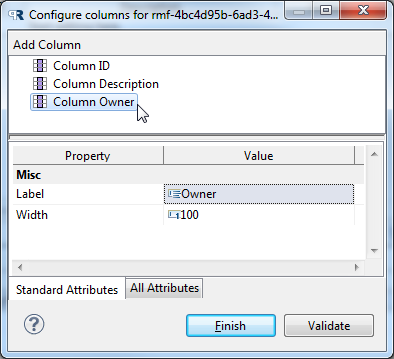
\includegraphics[width=0.8\linewidth]{../rmf-images/pror_column_configuration.png}      
\caption{Column Configuration}
\label{fig:column_configuration}
\end{figure}

Note that you have to provide Strings for the columns for the same
reason that we used Strings for the Labels earlier: This way we can
easily match multiple SpecObjects of different types.

You can actually adjust the width of the columns simply by dragging the
column headers.

\subsection{Adding new SpecObjects}

Now we can finally add SpecObjects by right-clicking on a row in the
Specification. In the context-menu, there are two submenus: ``New
Child'' and ``New Sibling''. ``New Child'' is the only way to produce a
hierarchical structure.

In both menus, there are three entries ``Spec Hierarchy'', ``Adding
SpecObjects'' and ``SpecObject (Requirement Type)''. Some background is
needed here:

We said before that Specifications contain references to SpecObjects. A
SpecHierarchy is the ``Wrapper'' that allows the hierarchical structure
and that points to the referred SpecObject. Usually, we don't have to be
concerned with them. Therefore the second option: If selected, a new
SpecHierarchy is created and associated with a new SpecObject, which in
turn is set immediately to the given SpecObjectType. If we had more than
just one SpecObjectType (besides ``Requirements Type''), there would be
an entry for each type in the context menu.

To continue the exercise, select the child ``SpecObject (Requirement
Type)''. Now we have two SpecObjects. Create a few more values and enter
some values. You can edit directly in the Specification, as you would in
Excel. Play around with Hierarchies.

You can drag and drop SpecObjects as a sibling or as a children. The
highlighting feedback helps you to find out whenever you shifting a
SpecObject as sibling or as a children. For instance, if you are
dragging a SpecObject over another one, the entire cell will be
highlighted. This means, that the SpecObject will be assigned as a
children to the dropped SpecObject.

\begin{figure}[h!]
\centering
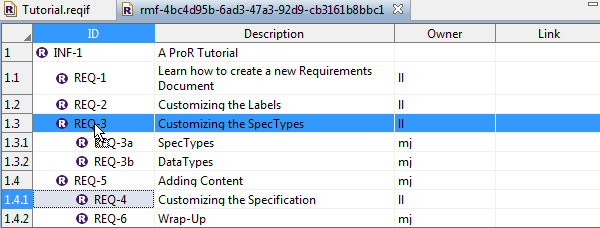
\includegraphics[width=\linewidth]{../rmf-images/feedback1.png}      
\caption{Drag and Drop as Child Object}      
\label{fig:dragAndDropChild}
\end{figure}

If you are dragging a SpecObject between two rows, you get also a visual
feedback an the SpecObject will be assigned as sibling:

\begin{figure}[h!]
\centering      
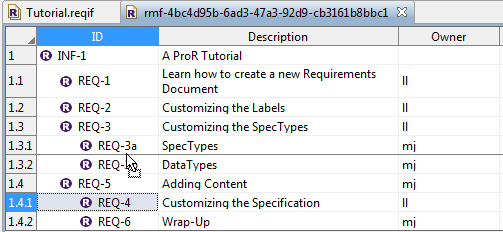
\includegraphics[width=0.8\linewidth]{../rmf-images/feedback2.png}      
\caption{Drag And Drop as Sibling Object}      
\label{fig:dragAndDropSibling}
\end{figure}

After some playing around, our Specification may look like this:

\begin{figure}[h!]
\centering      
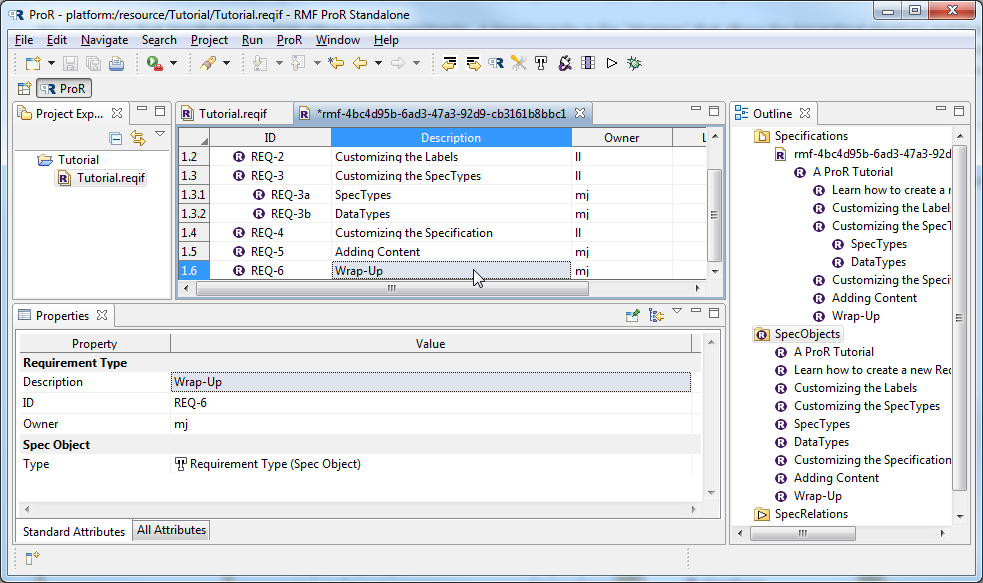
\includegraphics[width=\linewidth]{../rmf-images/pror_speceditor_2.png}      
\caption{Improved Specification}      
\label{fig:improvedSpec}
\end{figure}

\subsection{Export Specification as HTML}

If you want to export your Specification as HTML, go to ``File'' in the
main menu and click ``Print...''. The HTML representation is generated
and automatically opened in your default browser.

\subsection{Conclusion}

Quite an achievement - but also quite a bit of work to get started.
Also, entering information requires a lot of clicking, and some of the
descriptions are not completely visible. In the next part of the
tutorial, we will address these issues.

\section{Tutorial 2: Use Presentations}

We will continue where we left off with Tutorial 1 and we assume that
you have \pror{} in front of you with a similar model.

In this tutorial we will introduce Presentations. Presentations are
Eclipse Plug-Ins that extend the functionality of \pror{}. Specifically:

\begin{itemize}
\item
  Presentations can change the way how Attributes are rendered in the
  Specification
\item
  Presentations can change the way how Attributes are edited in the
  Specification
\item
  Presentations can perform tasks in the background.
\end{itemize}

\pror{} comes with a number of standard presentations that we will
introduce in this tutorial.

\subsection{Linewrap Presentation}

By default, text is not wrapped in cells. We will enable the Linewrap
Presentation for the Description column.

To do this, we select \pror{} \textgreater{} Presentation Configuration.

The dialog shown has no entries. The drop-down menu ``Select Action...''
at the top allows us to create new Presentations. We select the
``Linewrap'' Presentation. This will create a new entry in the upper
pane. Upon selecting it, we can configure it in the lower pane.

A Linewrap Presentation has only one configuration element, the
Datatype. We select ``T\_String32k''. This means that from now on, all
Attributes of this type will be rendered with the Linewrap Presentation.
Upon completion, the dialog should look like this:

\begin{figure}[h!]
\centering
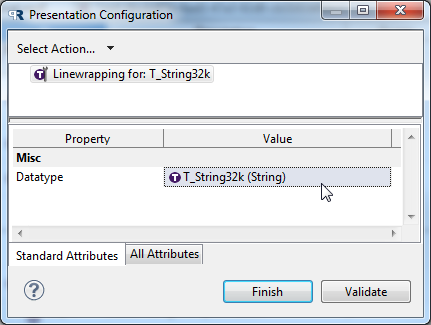
\includegraphics[width=0.8\linewidth]{../rmf-images/pror_presentation_configuration.png}      
\caption{Presentation Configuration Dialog}      
\label{fig:presentationConfig}
\end{figure}

Upon closing the dialog, the lines that are too long should be wrapped
automatically. Also, upon clicking on a cell, the content is now wrapped
in the editor.

\subsection{ID Presentation}

It would be nice if every SpecObject had its own unique ID. Actually, it
does (it is shown in the Property View, if a SpecObject is selected in
the Outline View). But that ID is meant for machines and is not
practical.

The ID Presentation allows the automatic creation of IDs. Let's create
one.

Remember that Presentations are associated with Datatypes, not
Attributes. Thus, we first have to create a new Datatype. We then
associate that Datatype with the Attribute ``ID''. We described this
process in the first tutorial. Here is a screen-shot of the
configuration dialog, when all is done:

\begin{figure}[h!]
\centering      
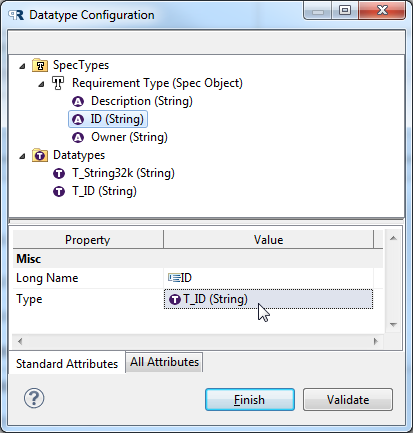
\includegraphics[width=0.8\linewidth]{../rmf-images/pror_id_configuration.png}      
\caption{Datatype Configuration Dialog}      
\label{fig:datatypeConfig}
\end{figure}

The last step is, like before, to associate that Datatype with the
Presentation.

We open the Presentation Configuration and create a new Presentation
from the dropdown menu ``Select Action...'', this time of type ``Id''
Presentation. We associate it with the newly created Datatype. After
configuration, the dialog should look as follows:

\begin{figure}[h!]
\centering      
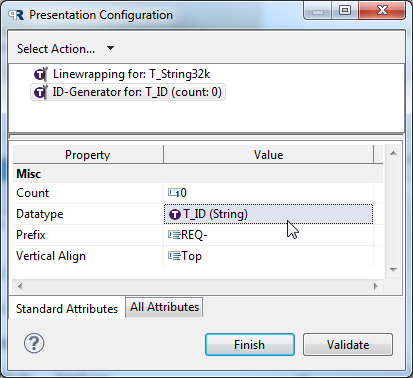
\includegraphics[width=0.8\linewidth]{../rmf-images/pror_id_presentation.png}      
\caption{ID Configuration Detail}      
\label{fig:idConfig}
\end{figure}

Note that you could adjust the prefix and the Count.

NOTE: At this point, the Presentation doesn't check yet for duplicates.
It simply grabs a new value from count, increments it and uses it. Also,
existing values are not overwritten.

\section{Tutorial 3: Advanced SpecTypes}

So far, we have a model with only one SpecObjectType. In this tutorial,
we will show how we can work with multiple SpecTypes, and we will
introduce other SpecTypes.

\subsection{Multiple SpecTypes}

The first entry in our Specification (``A \pror{} Tutorial'') isn't really
a requirement. Thus, it doesn't need an ID or an owner, and it would be
nice to Highlight it somehow. For Highlighting, we have the Headline
Presentation. We will:

\begin{itemize}

\item
  Create a new ``Headline'' SpecObjectType
\item
  Create a new Datatype that will be used for the Headline content
\item
  Associate that Datatype with the Headline Presentation
\end{itemize}

With \pror{} \textgreater{} Datatype Configuration we get the Dialog where
we can create new SpecTypes and Datatypes. For the first time, we create
a new SpecObjectType by right-clicking on ``SpecTypes''. One of the
entries in the child menu is ``SpecObject Type''.

Once created, we select it and rename to ``Headline Type'' it in the
properties.

Then we give it a new Attribute called ``Description''.

NOTE: It is important that we call it description. This matches the
Attribute from ``Requirement Type''. By using the same name, we ensure
that the Attributes appear in the same column, even though they are
different Attributes.

We do not set the type yet, as we need to create a new one. We do this
by right-clicking on ``Datatypes''. There we create a new ``Datatype
Definition String'' and call it ``T\_Headline''. Now we can go back to
the Description Attribute and set the type to T\_Headline.

When all this is done, the configuration should look like this:

\begin{figure}[h!]
\centering      
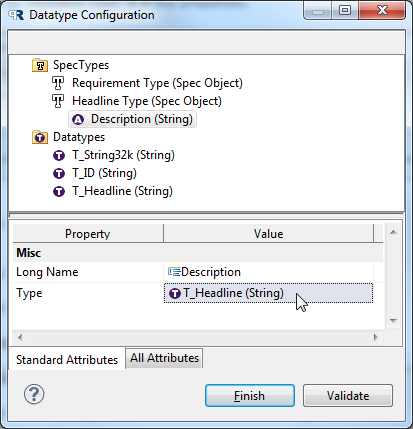
\includegraphics[width=0.8\linewidth]{../rmf-images/pror_datatype_headline1.png}      
\caption{Datatype Configuration for the Headline Presentation}      
\label{fig:headlineConfig}
\end{figure}

You can change the type of a SpecObject by selecting it an changing it
in the Properties view. Please note that currently all existing values
are lost when changing the type.

After the changes, the GUI should look as follows:

\begin{figure}[h!]
\centering      
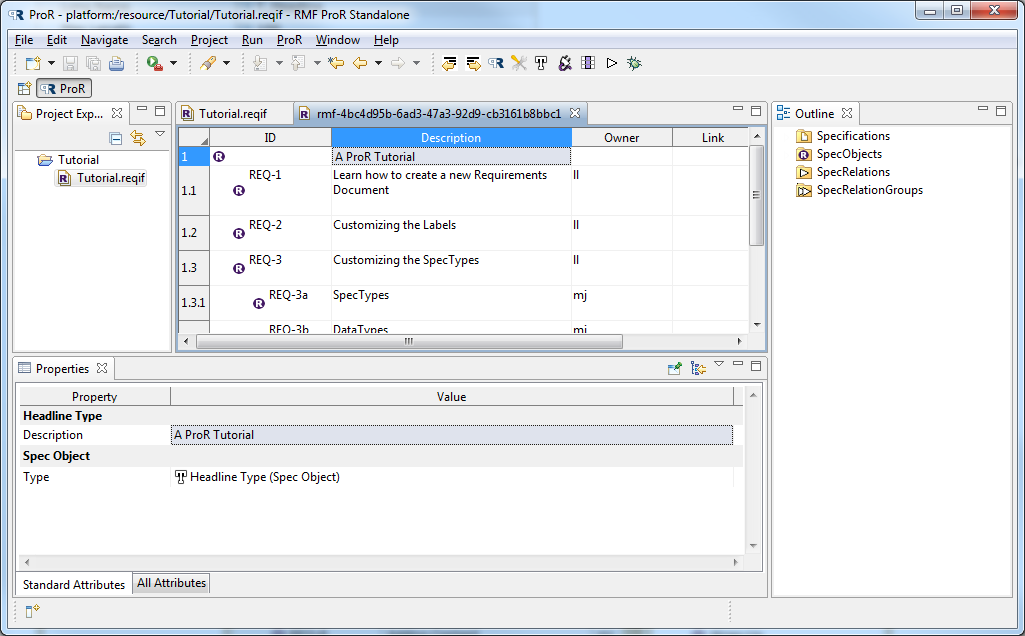
\includegraphics[width=\linewidth]{../rmf-images/pror_gui_with_headline.png}      
\caption{Activated Headline Configuration}      
\label{fig:activeHeadlineConfig}
\end{figure}

Note the following:

\begin{itemize}
\item
  The columns ``ID'' and ``Owner'' are now empty and cannot be edited
  for the Headline
\item
  Note how the Property View changes, as you select SpecObjects of
  different types
\item
  Right-clicking on a row now shows one more option for child/sibling
  creation: A new entry of type ``Headline Type''
\end{itemize}

Last, we will use the Headline Presentation for the type T\_Headline.
This is done via the Presentation Configuration, and should result in
the following. In addition, you can change the font size of the headline
in the ``Size'' Attribute:

\begin{figure}[h!]
\centering      
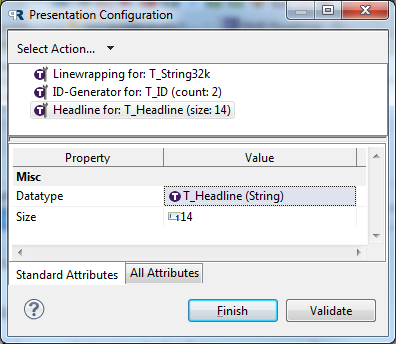
\includegraphics[width=0.8\linewidth]{../rmf-images/pror_datatype_headline2.png}      
\caption{Presentation Configuration for Headline}      
\label{fig:headlineConfig2}
\end{figure}

\subsection{Other SpecTypes}

You may have noticed in the Datatype Configuration Dialog, that
right-clicking on ``SpecTypes'' offered more options, besides ``Spec
Object Type''. A number of ReqIF-Elements can have Attributes.

We will now create a ``Specification Type'' and assign it to our
Specification.

Try to create a ``Specification Type'' and configure it as shown in the
screenshot:

\begin{figure}[h!]
\centering      
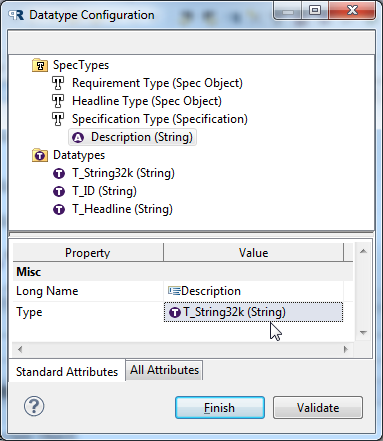
\includegraphics[width=0.8\linewidth]{../rmf-images/pror_new_spectype.png}      
\caption{Creating a New SpecType}      
\label{fig:newSpecType}
\end{figure}

Next, we will assign this type to the one Specification that we have. To
do this we select the Specification in the Outline View. That will show
the Specification's Properties in the Properties View. The ``Type''
Property is empty. We select ``Specification Type'' from the drop down.
As soon as it is selected, the Attribute ``Description'' will appear in
the properties view.

\section{Tutorial 4: Links between SpecObjects (SpecRelations)}

The implementation of SpecRelations is not complete yet. Still here are
a few pointers to show what is planned.

\subsection{Creating SpecRelations}

SpecRelations are created by ``Link-Dragging''. This is platform
specific:

\begin{itemize}

\item
  Linux: Dragging with Ctrl-Shift
\item
  Mac: ???
\item
  Windows: Dragging with Alt
\end{itemize}

Showing links as children can be switched on or off with the little
triangle icon in the toolbar:

\begin{figure}[h!]
\centering      
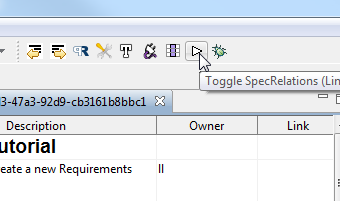
\includegraphics[width=0.8\linewidth]{../rmf-images/pror_toggle_links.png}      
\caption{Toggle Links on and off}      
\label{fig:toggleLinks}
\end{figure}

After creating a link:

\begin{itemize}
\item
  The ``Link'' column shows incoming and outgoing links
\item
  The SpecRelations are shown as children in the Specification view
\end{itemize}

SpecRelations can have their own Types. Once a type is set, the
corresponding columns in the Specification are rendered using
Presentations, etc. However. the Type has to be set explicitly (a link
created with dragging has currently no Type).

Here is a Screenshot of a Specification with some Links and a
SpecRelationType that includes a ``Description'' Attribute:

\begin{figure}[h!]      
\centering      
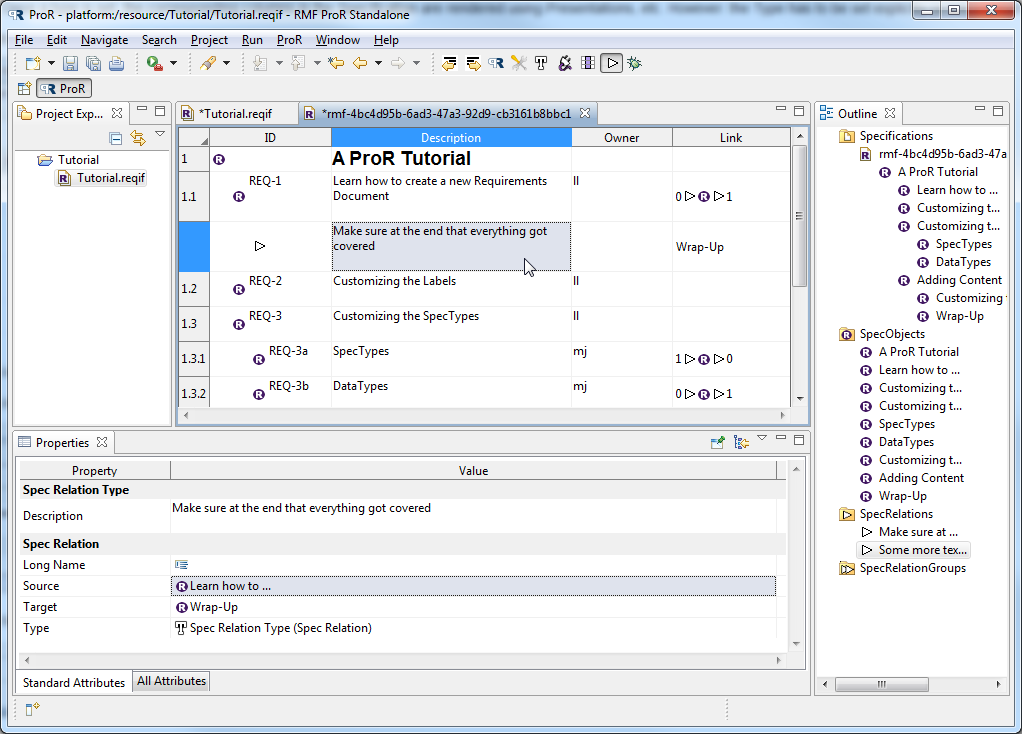
\includegraphics[width=\linewidth]{../rmf-images/pror_gui_with_links.png}      
\caption{Showing Links in the GUI}      
\label{fig:linksInGui}
\end{figure}

Note the following:

\begin{itemize}
\item
  The right column shows incoming and outgoing links
\item
  The number to the left of the triangle is incoming links, the other
  outgoing links
\item
  The outgoing link from REQ-1 is shown
\item
  The link from REQ-1 has a description, and it shows the destination
  name in the ``Link'' column
\end{itemize}

\subsection{Outline View}

Note that the Outline shows a folder with all SpecRelations.



\chapter{Reference}
%*******************************************************************************
% Copyright (c) 2014 Formal Mind GmbH and others
% All rights reserved. This program and the accompanying materials
% are made available under the terms of the Eclipse Public License v1.0
% which accompanies this distribution, and is available at
% http://www.eclipse.org/legal/epl-v10.html
% 
% Contributors:
%     Michael Jastram - initial Copy
%     Maha Jastram - susequent improvements
%******************************************************************************/

We hope you find this reference manual useful.  It's a work in progress and will be actively improved and expanded.

% ===================================================================================
\section{Editors}
% ===================================================================================

\begin{wrapfigure}{l}{.3\linewidth}
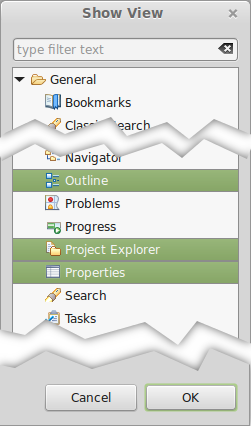
\includegraphics[height=.9\textwidth]{../rmf-images/views_highlighted.png}
\caption[flushleft]{Views.}
\label{fig:Views}
\end{wrapfigure}

Upon opening a ReqIF Model, the editor opens providing an overview of the model.  In essence what you are seeing is the Eclipse Workbench, with several modifications.  Here you will find a quick overview of each component.  A more detailed description of the Workbench can be found in Eclipse's Workbench User Guide.

A model contains any number of specifications, and the details of each specification can be inspected individually.  The windows in which all relevant information appears are called Views.  At your disposal are many Views with productivity, debugging, help and team resources.  We will be focusing only on the Views relevant to ProR.

% ===================================================================================
\subsection{ReqIF Overview Editor}
% ===================================================================================

This figure was briefly described in the tutorial.  Here we'll go deeper in depth.

\begin{figure}[h!]
  \centering
  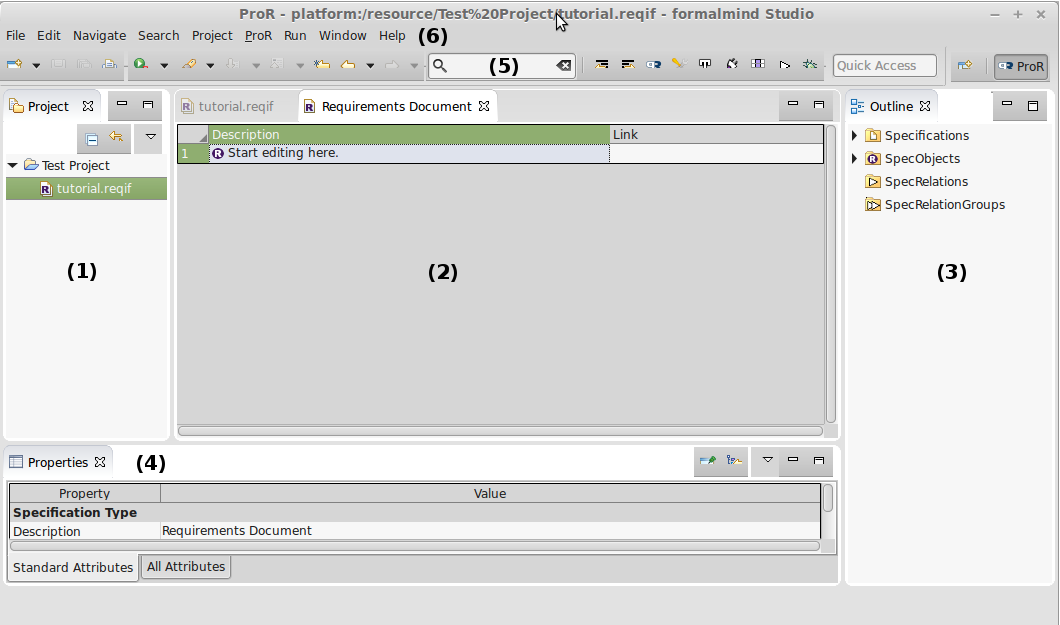
\includegraphics[width=\linewidth]{../rmf-images/Screenshot_intro.png}
  \caption{The \pror{} user interface}
  \label{fig:user_interface_overview}
\end{figure}

(1) is the Project Explorer window.  Here you will see a hierarchical listing of the project and the associated models.

(2) The Editor shows you a hierarchical breakdown of the model.  Each specification with it's associated SpecObjects is listed in a spreadsheet.  Because the SpecObjects of each requirement can vary, not all fields will be completed.  Because the fields need to  be created and then associated with the SpecObjects, they may not all be (nor do they need to be) represented.  But what appears and how they appear can be customized.

In the Editor, you see the SpecObjects that exist in this Specification.
There is currently only one, with the description "Start editing here".

The Outline (3) has four folders:

\begin{itemize}

\item
  "Specifications" shows the Specifications in the ReqIF.  You can
  expand the tree to expose the hierarchy of SpecObjects in the
  ReqIF model.
\item
  "SpecObjects" shows all SpecObjects in the ReqIF model as a flat list.
  Keep in mind that SpecObjects in Specifications are references.  In
  contrast, this folder shows all SpecObjects created for the ReqIF model, whether or not they are referenced.
\item
  "SpecRelations" shows all SpecRelations in the ReqIF as a flat list.
  For now, we will ignore SpecRelations.
\item
  "SpecRelationsGroups" represent an optional mechanism for grouping SpecRelations between two specific Specifications.
\end{itemize}

The properties of a selected Element are shown in the Properties view
(4).  As the only Requirement in the model is selected, we see its
SpecObjectType ("Requirements Type") and its only Attribute
("Description") with the value "Start editing here.".  There are two
tabs "Standard Attributes" and "All Attributes" at the bottom of the
Properties view.  ***** The "Standard Attributes" tab shows you all standard
attributes of the selected element.  The "All Attributes" shows all
existing ReqIF attributes of the selected element.

Above the main working windows it the tool bar (5) and, at the very top, the menu bar (6).
\subsection{Specification Editor}

% ===================================================================================
\section{Views}
% ===================================================================================

By default, ProR's Workbench displays the following three views:

\subsection{Project Explorer View}\index{Project Explorer View}

\subsection{Properties View}\index{Properties View}

\subsection{Outline View}\index{Outline View}

% ===================================================================================
\section{Configurations}
% ===================================================================================


The ProR menu contains entries to launch a number of configuration
dialogs.

\subsection{General Configuration}\index{Configuration!General}

\subsection{Datatype Configuration}\index{Configuration!Datatype}

This configuration is opened via ProR \textbar{} Datatype Configuration
...

The dialog shows two folders, one for SpecTypes and one for Datatypes.
SpecTypes are created for typing elements that have attributes
(SpecObjects, Specifications, SpecRelations).  New SpecTypes can be
created by right-clicking on the folder and selecting ``New Child''.
Through the same mechanism, attribute definitions can be added to a
SpecType.  attribute definitions are typed.  Selecting an element shows
its properties in the lower pane, where it can be configured.

Attribute definitions must have a name and a datatype.  Some attribute
definitions allow further customization.  The datatype is selected from a
dropdown.  New datatypes can be created by right-clicking on the folder
``Datatypes'' and selecting ``New Child''.  Again, selecting a datatype
shows its properties in the lower pane, where it can be configured.  A
datatype should have at least a long name.

As an example, consider the following Datatype Configuration Dialog:

\begin{figure}[h!]
\centering     
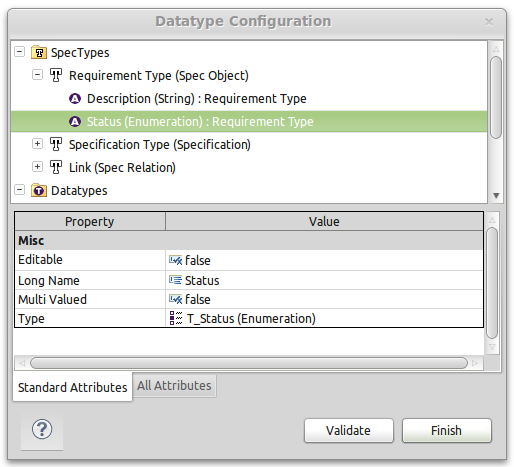
\includegraphics[width=0.8\linewidth]{../rmf-images/pror_datatype_configuration.png}
\caption{Datatype Configuration Dialog}      
\label{fig:DatatypeConfig}
\end{figure}

The Spec Type for ``Requirements Type'', which is applicable to
SpecObjects, is expanded.  The Spec Type has two attributes,
``Description'' (String) and ``Status'' (Enumeration).  Status is
selected, and in the pane below the mandatory values, ``Long Name'' and
``Type'' have been set.  Further customization of the attribute is
possible, e.g.  by converting it in a Multi-Valued attribute by setting
the corresponding flag to ``true''.

\subsubsection{Enumeration Datatypes}

An enumeration datatype must have enumeration values.  These are created
by right-clicking the enumeration datatype and selecting New Child
\textbar{} Enum Value.  You may have to unfold the enum value to select
it, so that you can provide it with a Long Name.  The following shows a
correctly configured enumeration datatype:

\begin{figure}[h!]
\centering      
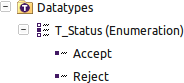
\includegraphics[width=0.4\linewidth]{../rmf-images/rmf_enumeration.png}
\caption{Enumerations}      
\label{fig:Enumerations}
\end{figure}

\subsection{Presentation Configuration}\index{Configuration!Presentation}

\subsection{Column Configuration}\index{Configuration!Column}

This configuration is specific to the Specification Editor.

The Column Configuration Dialog configures the Columns of a
Specification.  Columns are identified by name.  The width of the column
can be adjusted directly by dragging the column separator in the table
header.

If the SpecObject has an attribute where the name of the attribute
matches the name of the column, then that attribute is shown in that
column.


\chapter{Presentations}
%*******************************************************************************
% Copyright (c) 2014 Formal Mind GmbH and others
% All rights reserved. This program and the accompanying materials
% are made available under the terms of the Eclipse Public License v1.0
% which accompanies this distribution, and is available at
% http://www.eclipse.org/legal/epl-v10.html
% 
% Contributors:
%     Michael Jastram - initial Copy
%     Maha Jastram - subsequent improvements
%******************************************************************************/

\pror{} has an extension mechanism that allows custom rendering, custom editing and automatic modifications to the requirements model. These extensions are called \term{presentations}.

Presentations can be created and configured via \menu{ProR | Presentation Configuration...} or the icon 
\includegraphics[height=1em]{../rmf-images/icons/full/obj16//ReqIFToolExtension.png} in the toolbar.  Launching it will show the dialog shown in Figure~\ref{fig:presentation-dialog}.  Initially, the dialog will be empty.  The dialog in the figure shows two presentation configurations.

Presentations are specific for a model, and its configuration is also stored in the requirements model.

\pror{} ships with a small set of standard presentations.  Additional presentations can be installed into \pror{}.

\begin{warning}
Note that presentations are specific to \pror{}, not to ReqIF.  This means that other tools will simply ignore presentations.  Also note that the behavior of the tool is unpredictable if a presentation used by a model is not installed in \pror{}.
\end{warning}

\begin{figure}
  \centering
  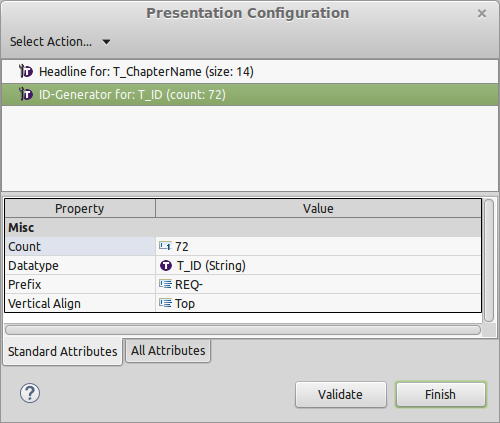
\includegraphics[width=0.8\textwidth]{../rmf-images/presentation-dialog.png}
  \caption{The presentation dialog with two configured presentations}
  \label{fig:presentation-dialog}
\end{figure}

% ===================================================================================
\section{Working with Presentations}
\index{presentation dialog}
% ===================================================================================

All presentations are configured in the same way.  To configure a presentation for the current model, first open the presentation configuration dialog as described above.

Initially, the dialog is empty.  You can add new presentations using the \menu{Select Action...} dropdown.  It will list all built-in and installed presentations.  Upon selecting an entry, it will be added to the list below.

\begin{info}It is possible (and often useful) to add the same presentation multiple times. For instance, one could add multiple ID generation presentations for different types of elements (with correspondingly different prefixes). 
\end{info}

Selecting a presentation in the upper pane will show its configuration parameters in the lower pane.  In Figure~\ref{fig:presentation-dialog}, the ID-Generator is selected, and the lower pane shows its four configuration parameters.

All presentations have a configuration parameter \menu{Datatype}.  Typically, the datatype determines whether a presentation is applied to an element or not.

\begin{info}
  If you want a presentation to be applied to a dedicated \term{Attribute} (rather than \term{Datatype}, then simply create a specific datatype for that attribute. And conversely, you can reuse a single presentation for multiple attributes by using the same datatype for all relevant Attributes.
\end{info}

The order of entries sometimes (but rarely) matters.  Presentations can be reordered using drag and drop.

Last, to delete a presentation, select \menu{Delete} from the context menu by right-clicking.

% ===================================================================================
\section{Default Datatype Handlers}
\index{presentations!default handlers}
\index{default handlers}
% ===================================================================================

Sometimes, it is desirable to use a presentation as the default for rendering (and editing) a specific datatype.  For example, the open source ProR can not render formatted (XHTML) text and instead shows a simplification in plain text.  But formalmind Studio offers the RTF presentation that allows rich rendering and editing.  Thus, it would be nice if XHTML datatypes would always be rendered using the RTF presentation, if installed.

This is possible.  And in fact, presentations can request to be used as default handlers.  If such a presentation is installed, it will automatically take over from the default.

Users can configure and override this.  To do so, go to \menu{Window | Preferences | ProR | Default Presentations}.  The resulting dialog is shown in Figure~\ref{fig:default-handlers}.

\begin{figure}
  \centering
  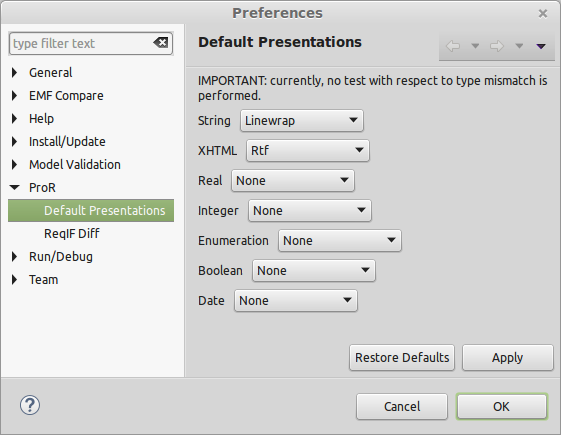
\includegraphics[width=0.8\textwidth]{../rmf-images/default-handlers.png}
  \caption{The preference dialog for handling default presentations}
  \label{fig:default-handlers}
\end{figure}

For each of the standard ReqIF datatypes, a handler can be chosen.  The default is \menu{none}.  The following entries are available:

\begin{description}
\item[None.] This is the default and implies that the build-in renderer is used.   Upon starting the tool, \pror{} will check whether a new presentation has been installed that requests to act as the default handler for that datatype.  If such a presentation is found, it will be set as the handler.
\item[Use Built-in.] This forces the built-in handler to be used.  Even if an installed presentation requests to be the handler, the built-in handler will continue to be used.
\item[List of installed presentations.] The remaining entries list all installed presentations.  Note that the dialog does not filter the matching types.  I.e. even though the RTF presentation is only applicable for XHTML, it is shown in the dropdown for all datatypes.
\end{description}

\begin{warning}
Please make sure that you only set datatype handlers of the correct type.  Also note that there is no access to the configuration parameters of default handlers. Therefore, this mechanism makes only sense for presentations that do not require any additional configuration.
\end{warning}

% ===================================================================================
\section{Built-in ProR Presentations}
\index{presentations!build-in ProR}
% ===================================================================================

The following presentations are part of the Eclipse RMF project and are therefore open source.

% -----------------------------------------------------------------------------------
\subsection{ID Generator Presentation}
\index{presentation!id generator}
\label{sec:id_presentation}
% -----------------------------------------------------------------------------------

This presentation automatically generates user-friendly IDs, consisting of a prefix and a number, e.g. ``REQ-12''. The configuration parameters are shown in Figure~\ref{fig:default-handlers}.

\begin{info}
Attributes to which this presentation applies are read-only and cannot be edited manually any more (as long as the presentation is active).
\end{info}

The parameters are:

\begin{description}
\item[Count.] The counter position. When a new ID is created, it will be incremented by one.  Changing it allows  the user to start or continue with a different number.
\item[Datatype.] The presentation will be applied to all attributes with this datatype.  Must by of type \term{String}.
\item[Prefix.] The prefix to the number.  Note that changing this will only modify newly created IDs, not those already generated.
\item[Vertical align.] Allows to adjust how the text shall be rendered in the cell.
\end{description}

\begin{warning}
Currently, the presentation does not check whether duplicate IDs exist!
\end{warning}

% -----------------------------------------------------------------------------------
\subsection{Headline Presentation}
\index{presentation!headline}
% -----------------------------------------------------------------------------------

This presentation renders the content of a cell boldface in a large font.  This can be useful if
you want to format text to stand out (e.g. a headline), without having to resort to XHTML.

The parameters are:

\begin{description}
\item[Datatype.] The presentation will be applied to all attributes with this datatype.  Must by of type \term{String}.
\item[Size.] The size of the text in point.
\end{description}

% -----------------------------------------------------------------------------------
\subsection{Linewrap}
\index{presentation!linewrap}
% -----------------------------------------------------------------------------------

This presentation wraps text at word boundaries, essentially what one would expect anyway.  The built-in renderer breaks the text anywhere, including in the middle of words.

This presentation is usually set as the default presentation.

\begin{info}
Regular users can just ignore this presentation.  It has been created for developers to understand the presentation mechanism.
\end{info}



\chapter{Glossary}
\section{ReqIF}

ReqIF stands for Requirements Interchange Format.  It is an exchange format for requirements and a data model.  ReqIF is the successor of \href{RMF/RIF}{RIF} and an OMG standard.

RMF supports ReqIF 1.0.1 (\href{http://www.omg.org/spec/ReqIF/}{official OMG standard}).

The \href{RMF/ProR}{ProR} GUI does support ReqIF.

\subsection{History}

For technical and organizational reasons, two companies in the manufacturing industry are rarely able to work on the same requirements repository and sometimes do not work with the same requirements authoring tools.  A generic, non-proprietary format for requirements information is required to cross the chasm and to satisfy the urgent industry need for exchanging requirement information between different companies without losing the advantage of requirements management at the organizations' borders.

The Requirements Interchange Format (ReqIF) described in this RFC defines such a tool-independent exchange format.  Requirement information is exchanged by transferring XML documents that comply to the ReqIF format.

In 2004, the HIS (Hersteller Initiative Software), a panel of Germany's automotive manufacturers (Daimler, VW, Porsche, Audi and BMW Group) developed the idea of creating the ``Requirements Interchange Format''.  In 2005, the first version of that format was presented at the REConf®, a conference about requirements engineering and management, in Munich.  In 2008, the HIS Steering Committee decided that the internationalization and maintenance of the Requirements Interchange Format should be proceeded with the ProSTEP iViP Association.  A project was set up and a team was built that includes members of the ProSTEP iViP Association, representatives of manufacturing companies (Audi, BMW  Group, Daimler, VW, Bosch and Continental), tool vendors (Atego, IBM, MKS) and development partners (HOOD GmbH, PROSTEP AG).

The ReqIF team expects that making the Requirements Interchange Format an OMG standard increases the number of interoperable exchange tool implementations on the market, fosters the trust of companies exchanging requirement information in the exchange format and provides safety of investments to tool vendors.

\subsection{Previous Versions of ReqIF}

This document is submitted as RFC of the Requirements Interchange Format (ReqIF) to the OMG.  Before the submission, the Requirements Interchange Format has been a specification proposed by the HIS and in its latest version, a recommendation of ProSTEP iViP.  For these versions, the abbreviation ``RIF'' has been applied.  The HIS released the Requirements Interchange Format as RIF 1.0, RIF1.0a, RIF 1.1; RIF1.1a and the ProSTEP iViP released the recommendation RIF 1.2.

As the acronym RIF has an ambiguous meaning within the OMG, the acronym ReqIF has been introduced to separate it from the W3C`s Rule Interchange Format.  ReqIF 1.0 is the direct successor of the ProSTEP iViP recommendation RIF 1.2.

\section{RIF}

RIF stands for Requirements Interchange Format.  It is an exchange format for requirements and a data model.  RIF is the predecessor of \href{RMF/ReqIF}{ReqIF}.

RMF supports the following versions of RIF:

\begin{itemize}
\item RIF 1.1a
\item RIF 1.2
\end{itemize}

The ProR GUI does currently not support RIF.

\section{Eclipse}

\subsection{Committer License Agreement (CLA)}\index{Committer License Agreement}

The Committer License Agreement (CLA) needs to be signed by contributors to Eclipse projects.  It essentially states that you hold all rights to your contribution and that you allow Eclipse to use them under the Eclipse Public License.




\end{document}

